\chapter{Media Transmisi}

Media transmisi adalah jalur fisik antara transmitter dan receiver di sistem transmisi data. Pada bab sebelumnya telah dijelaskan bahwa gelombang elektromagnetik dipandu sepanjang media solid di media terpandu (\textbf{guided media}). Contohnya seperti copper twisted pair, copper coaxial cable dan fiber optik. Sedangkan transmisi nirkabel terjadi melalui atmosfer, luar angkasa atau air di media tak terpandu (\textbf{unguided media})

Karakteristik dan kualitas dari transmisi data ditentukan oleh katakteristik medium dan karakteristik sinyalnya. Pada media terpandu, medium itu sendiri merupakan hal terpenting yang dapat menentukan batasan transmisi. Pada media tak terpandu, bandwidth dari sinyal yang dihasilkan oleh antena transmisi lebih penting dari pada medium dalam penentuan karakteristik transmisi.

Salah satu sifat sinyal yang ditransmisikan melalui antena adalah directionality. Secara umum, sinyal pada frekuensi lebih rendah adalah omni-directional artinya sinyal berpropagasi ke segala arah. Sedangkan pada frekuensi lebih tinggi, sinyal dapat difokuskan menjadi directional beam.

Data rate dan jarak menjadi salah satu pertimbangan dalam desain sistem transmisi data. Tujuannya adalah dicapainya data rate yang tinggi dan jarak jangkauannya yang jauh.  Beberapa faktor dari media transmisi dan sinyal yang menentukan data rate dan jarak jangkauannya adalah sebagai berikut

\begin{itemize}
	\item \textbf{Bandwidth:} Semakin besar bandwidth sinyalnya maka semakin besar data rate yang dapat dicapai.
	\item \textbf{Transmission impairment/ kerusakan transmisi: } Impairments seperti atenuasi dapat membatasi jarak. Pada media terpandu, twisted pair umumnya lebih rentan terhadap impairment daripada coaxial cable dan coaxial cable lebih rentan terhadap impairment daripada fiber optic.
	\item \textbf{Interference:} Interference dari sinyal lain pada overlapping frequency band dapat mendistorsi atau meng-cancel out sinyal tersebut. Umumnya interference terjadi di media tak terpandu, tapi juga terkadang di media terpandu. Pada media terpandu, interference dapat disebabkan alien crosstalk (antar kabel) maupun internal crosstalk (antar konduktor dalam satu cable sheath). Sedangkan pada media tak terpandu, interference disebabkan oleh electromagnetic coupling. Untuk meminimalkan interference pada media terpandu, gunakan shield yang baik.
	\item \textbf{Jumlah receiver:} Media terpandu dapat digunakan untuk membangun transmisi point-to-point link atau shared link dengan banyak attachment. Setiap attachment ini yang akan memberikan atenuasi maupun distorsi, batasan jarak dan/atau data rate.
\end{itemize}

Gambar \ref{fig:4.1.spectrum_em_telecom} menunjukkan grafik spektrum gelombang elektromagnetik dimana setiap media transmisi, baik media terpandu maupun tak terpandu, beroperasi.

\begin{figure}
	\centering
	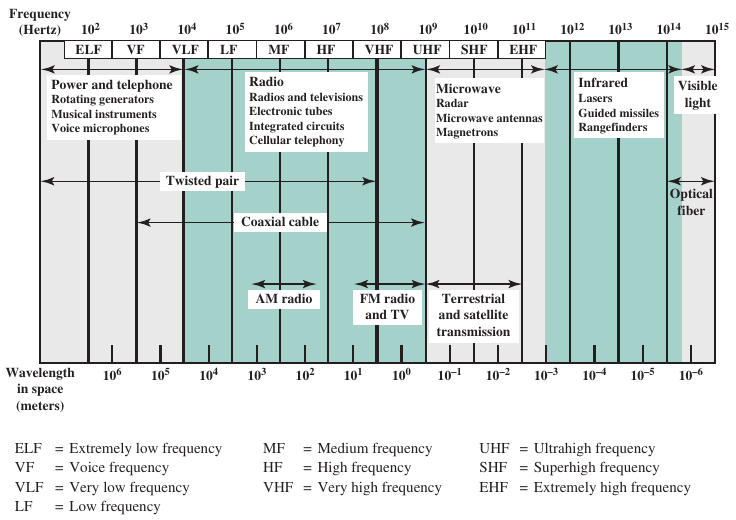
\includegraphics[width=1\linewidth]{gambar/4.1.gambar.4.1.spectrum_emw_media_transmisi}
	\caption{Spektrum gelombang elektromagnetik dari telekomunikasi}
	\label{fig:4.1.spectrum_em_telecom}
\end{figure}

\section{Media Transmisi Terpandu/ Guided Transmission Media}

Pada media transmisi terpandu, kapasitas transmisi, baik dalam data rate maupun bandwidth, bergantung pada jarak dan bentuk transmisinya, apakah point-to-point atau multipoint seperti yang ditunjukkan oleh Gambar \ref{fig:4.table_point_to_point}. Tiga media terpandu yang biasanya digunakan adalah twisted pair, kabel koaksial, dan fiber optik seperti yang ditunjukan oleh Gambar \ref{fig:4.media.terpandu}

\begin{figure}
	\centering
	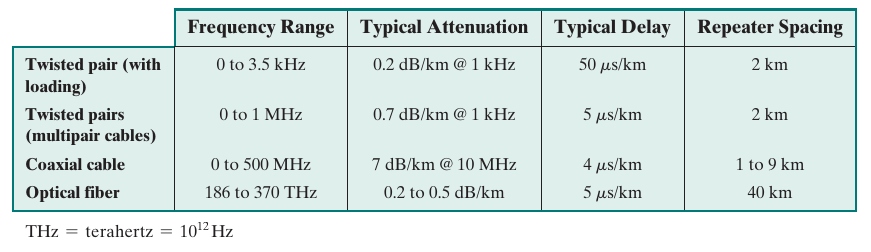
\includegraphics[width=1\linewidth]{gambar/4.1.table_4.1.point_to_point_characteristics}
	\caption{Karakteristik transmisi point-to-point dari media terpandu}
	\label{fig:4.table_point_to_point}
\end{figure}

\begin{figure}
	\centering
	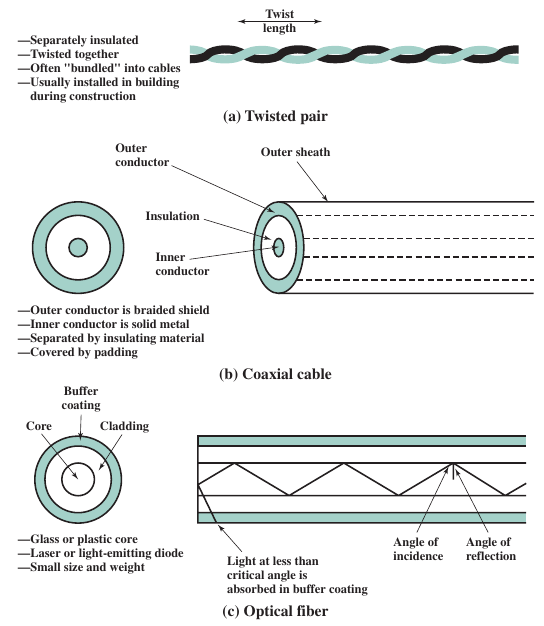
\includegraphics[width=\linewidth]{gambar/4.1.gambar.4.2.media_terpandu}
	\caption{Media transmisi terpandu}
	\label{fig:4.media.terpandu}
\end{figure}

\subsection{Twisted-pair}

Twisted-pair paling banyak digunakan di media transmisi terpandu dan harganya murah.

\subsubsection{Deskripsi fisik}

Twisted pair terdiri dari 2 insulated copper wire yang diatur dengan pola spiral. Setiap twisted-pair bertindak sebagai satu communication link. Twisted-pair dibungkus bersama di dalam protective sheath/jacket. Untuk mendapatkan jarak yang lebih jauh, biasanya terdiri dari ratusan twister-pair. Twisting dilakukan untuk meminimalkan crosstalk. A

\section{Transmisi Nirkabel}

\section{Propagasi Nirkabel}

\section{Transmisi Line-of-sight}

